\documentclass[paper=a4,fontsize=11pt]{report} % A4 paper and 11pt font size

\usepackage[T1]{fontenc} % Use 8-bit encoding that has 256 glyphs
\usepackage{fourier} % Use the Adobe Utopia font for the document - comment this line to return to the LaTeX default
\usepackage{graphicx} % For pictures
\usepackage{booktabs} % For tables
\usepackage{tabularx} % For tables
\usepackage[english]{babel} % English language/hyphenation
\usepackage{amsmath,amsfonts,amsthm} % Math packages

\usepackage[margin=1.5in]{geometry}

\usepackage{lipsum} % Used for inserting dummy 'Lorem ipsum' text into the template

\usepackage{sectsty} % Allows customizing section commands
\allsectionsfont{\centering \normalfont\scshape} % Make all sections centered, the default font and small caps

\usepackage{fancyhdr} % Custom headers and footers
\pagestyle{fancyplain} % Makes all pages in the document conform to the custom headers and footers
\fancyhead{} % No page header - if you want one, create it in the same way as the footers below
\fancyfoot[L]{} % Empty left footer
\fancyfoot[C]{} % Empty center footer
\fancyfoot[R]{\thepage} % Page numbering for right footer
\renewcommand{\headrulewidth}{0pt} % Remove header underlines
\renewcommand{\footrulewidth}{0pt} % Remove footer underlines
\setlength{\headheight}{13.6pt} % Customize the height of the header

\numberwithin{equation}{section} % Number equations within sections (i.e. 1.1, 1.2, 2.1, 2.2 instead of 1, 2, 3, 4)
\numberwithin{figure}{section} % Number figures within sections (i.e. 1.1, 1.2, 2.1, 2.2 instead of 1, 2, 3, 4)
\numberwithin{table}{section} % Number tables within sections (i.e. 1.1, 1.2, 2.1, 2.2 instead of 1, 2, 3, 4)

% \setlength\parindent{0pt} % Removes all indentation from paragraphs - comment this line for an assignment with lots of text

\renewcommand{\thesection}{\arabic{section}}

%----------------------------------------------------------------------------------------
%	TITLE SECTION
%----------------------------------------------------------------------------------------

\newcommand{\horrule}[1]{\rule{\linewidth}{#1}} % Create horizontal rule command with 1 argument of height

\title{	
\normalfont \normalsize 
\textsc{Georgia Institute of Technology} \\ [25pt] % Your university, school and/or department name(s)
\horrule{0.5pt} \\[0.4cm] % Thin top horizontal rule
\huge CS 6210 Project 2 Report: Shared Memory IPC \\ % The assignment title
\horrule{2pt} \\[0.5cm] % Thick bottom horizontal rule
}

\author{Manas George, Paras Jain} % Your name

\date{\normalsize\today} % Today's date or a custom date

\begin{document}

\maketitle % Print the title

\section{Project goal}
TinyFile is a service that accepts files through shared-memory IPC and then compresses/decompresses the data. Clients can communicate with the service and offload the work of compression to TinyFile. Behind TinyFile is an implementation of the \texttt{snappy} compression protocol.

In order to support inter-process communication between clients and the server, both a blocking and asynchronous interfaces are availible for end users. This interface allows for data to be efficiently shuttled between the client and server process through shared memory.

\section{TinyFile Architecture}
The TinyFile application is structured as a client-server program. The server is a standalone daemon that accepts requests to compress files from clients. The client is a library that is linked into client applications that need to use the application. Client applications call exported functions from the client library to send data they want compressed to the compression server running separately as a daemon, which responds with the compressed version of the file.

\subsection{Server Design}
The server \texttt{bin/tinyd} allows users to start a daemon which listens for incoming compression requests. After initialization, the server alternates between servicing client requests to join/leave the service and actual compression requests.

\subsubsection{Data Structures}
The server maintains state for each client it is currently communicating with, and calls out to the snappy-c library to actually perform the requested compression. Client state is tracked in a linked-list structure that records, for each client, the private message queue and the shared memory segment used to perform client-server communication.

\begin{figure}[b!]
  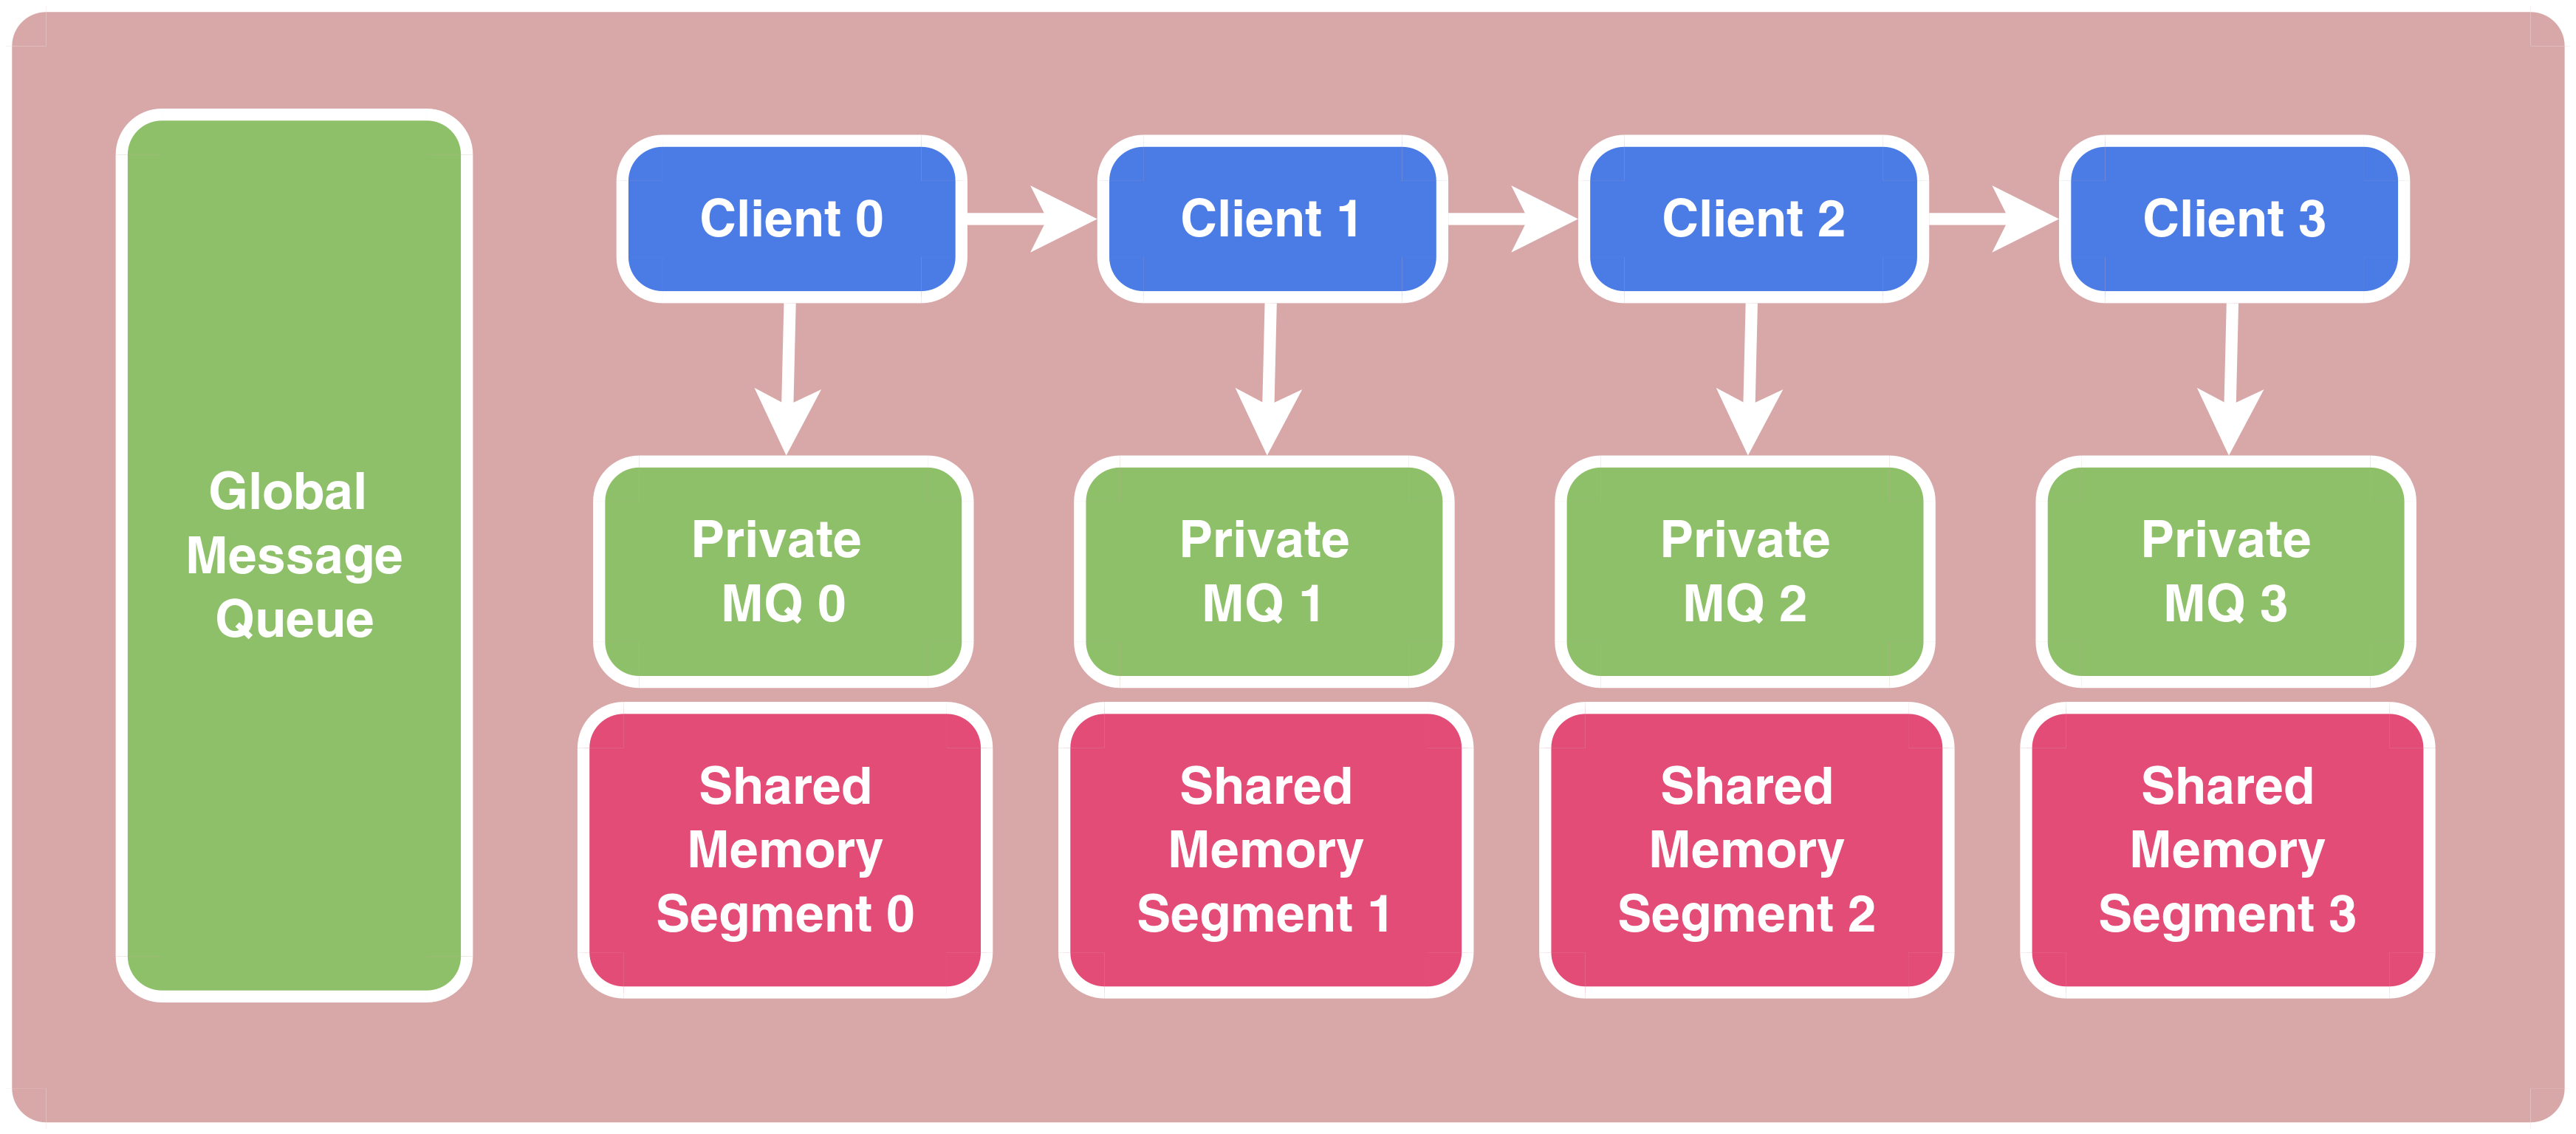
\includegraphics[width=\linewidth]{img/ll.png}
  \caption{Server data structures}
\end{figure}

Apart from private message queues for each client, the server also has a global shared message queue that is available to all clients. This queue is used to initialize clients, as described in the following section, and for nothing else. Requests to join/leave the service can therefore be handled independently from actual service IPC traffic.

\subsubsection{Client Initialization}
When a new client comes online, it must register with the server using the \texttt{tiny\_initialize} function exported by the library. The initialization function uses the global shared message queue to send an initialization request to the server, invoking a series of initialization procedures on the server side that comprise the initial client-server handshake.

\begin{figure}[b!]
  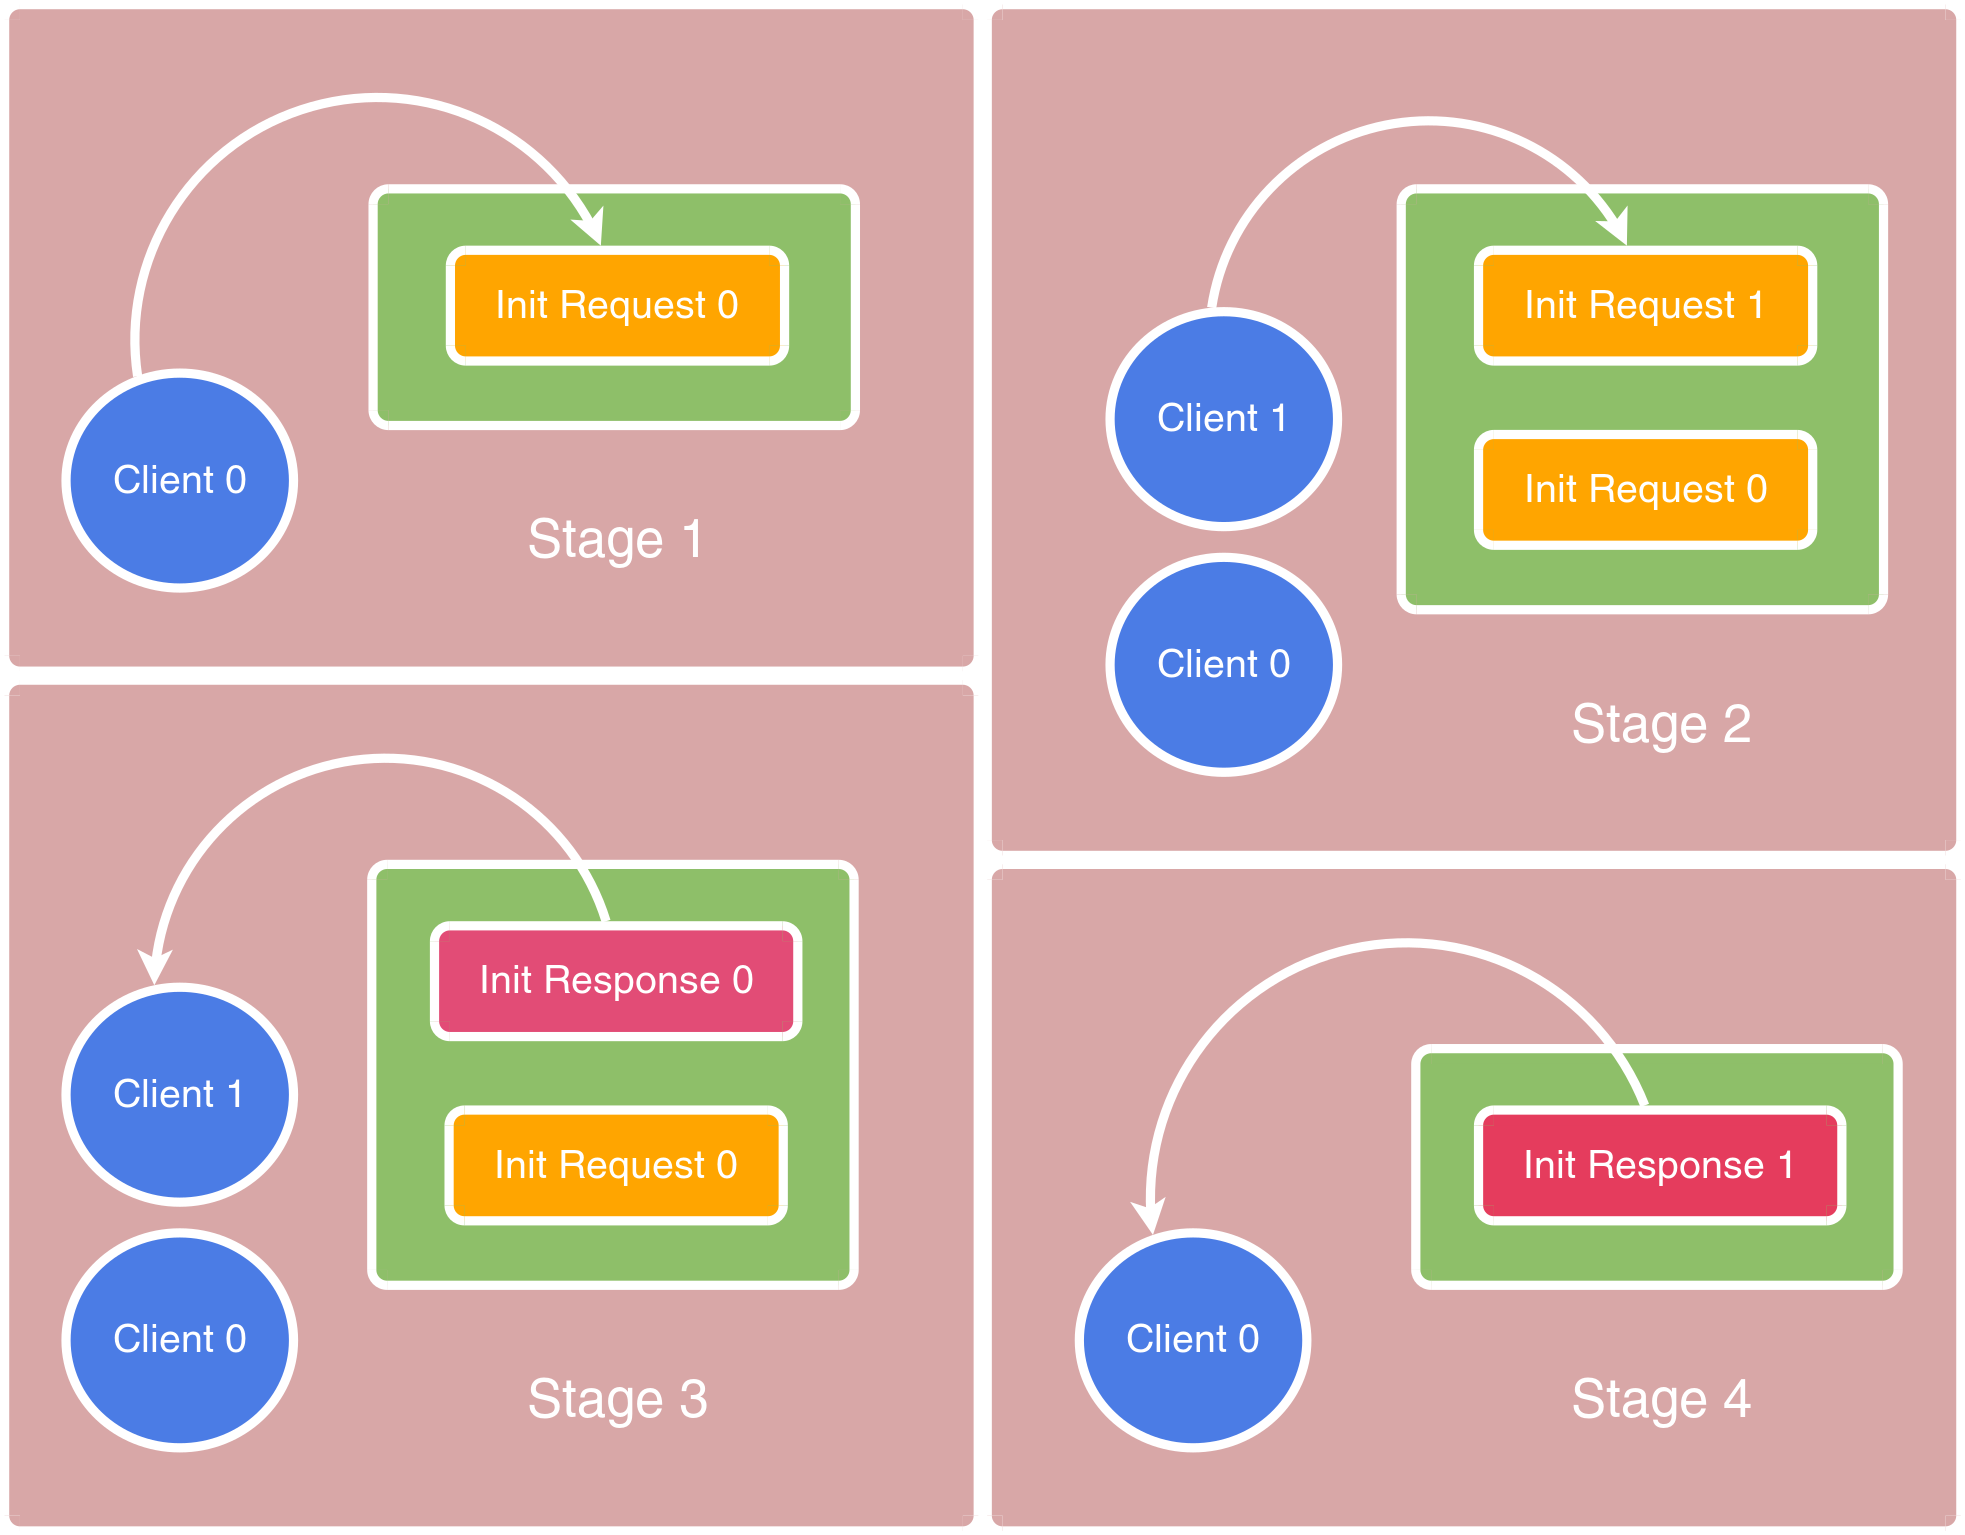
\includegraphics[width=\linewidth]{img/init.png}
  \caption{Initialization race condition}
\end{figure}

\begin{enumerate}
\item Memory is allocated to store the new client's state.
\item The client is assigned new unique id and a temporary file.
\item The temporary file is used to derive an IPC key.
\item The IPC key is used to initialize a private message queue and shared memory.
\item The new client is placed at the head of the global clients list.
\end{enumerate}

Once all of this is done, the server responds with a message that contains the \texttt{client\_key} created from the client's temporary file, which is the only information the client needs to connect to its private message queue and shared memory segment. The initialization request and response are sent over the global shared message queue common to all clients. This introduces the possibility of a race condition in since there is no guarantee that a particular response will reach exactly the client it was sent from. This is not really a problem, as the clients are essentially indistinguishable until the handshake is completed, and so a situation in which a client reads an initialization response message intended for another client is never problematic; the original client will simply receive a response message intended for yet another client, and all clients end up with unique IDs and keys in the end. Notice that mixing up of messages is not an issue once the handshake is done. The global shared message queue is only used for initialization; all subsequent messages between a server and client go through a per-client client-private message queue that is initialized during the handshake.

\subsubsection{Compressing/Uncompressing Data}
Once the client link is established, each client can communicate over its own message queue with the server. This private line contains requests from the client to the server to process a request. Service data is delivered through the shared memory and a response is finally communicated back through the shared store.

Specifically, the process of compressing a file using the blocking API is as follows:
\begin{enumerate}
\item The client reads the file into a buffer
\item Client calls \texttt{tiny\_compress}, passing in the buffer and file size
\item The client library places the relevant arguments in the shared memory header \texttt{shm\_header} and then copies the file buffer into the shared memory space
\item The client library then sends a message to the server to request decompression
\item When the server main loop services the relevant client queue, it invokes snappy to compress the buffer. It then copies the result back into shared memory.
\item The server notifies the client that compression occurred through shared memory
\item The client can copy the resulting compressed file from shared memory, thus freeing the region for use in the next call
\end{enumerate}

\subsubsection{Cleaning Up}

Clients degister themselves by sending a message on the main server IPC queue (not the private queue). The server recieves the message off the bus and then deallocated relevant data structures. This includes closing the message queue and and marking the shared memory region for deletion. Clients can then quit. When a \texttt{ctrl-c} signal is recieved, the system cleans up after each client before exiting safely.

\section{API}

\section{Performance}

\end{document}